\documentclass[12pt]{article}
\usepackage{graphicx}
\usepackage{float} 

\begin{document}
	\begin{center}
		\LARGE{Stiffness model for Tripteron robot}
	\end{center}
	\section{Virtual Joints model}
	\begin{itemize}
		\item Consider each of three legs separately. The model for them are same the only difference is axis of rotations and translations of links and joints.\\
		Model scheme:
		\begin{figure}[H]
			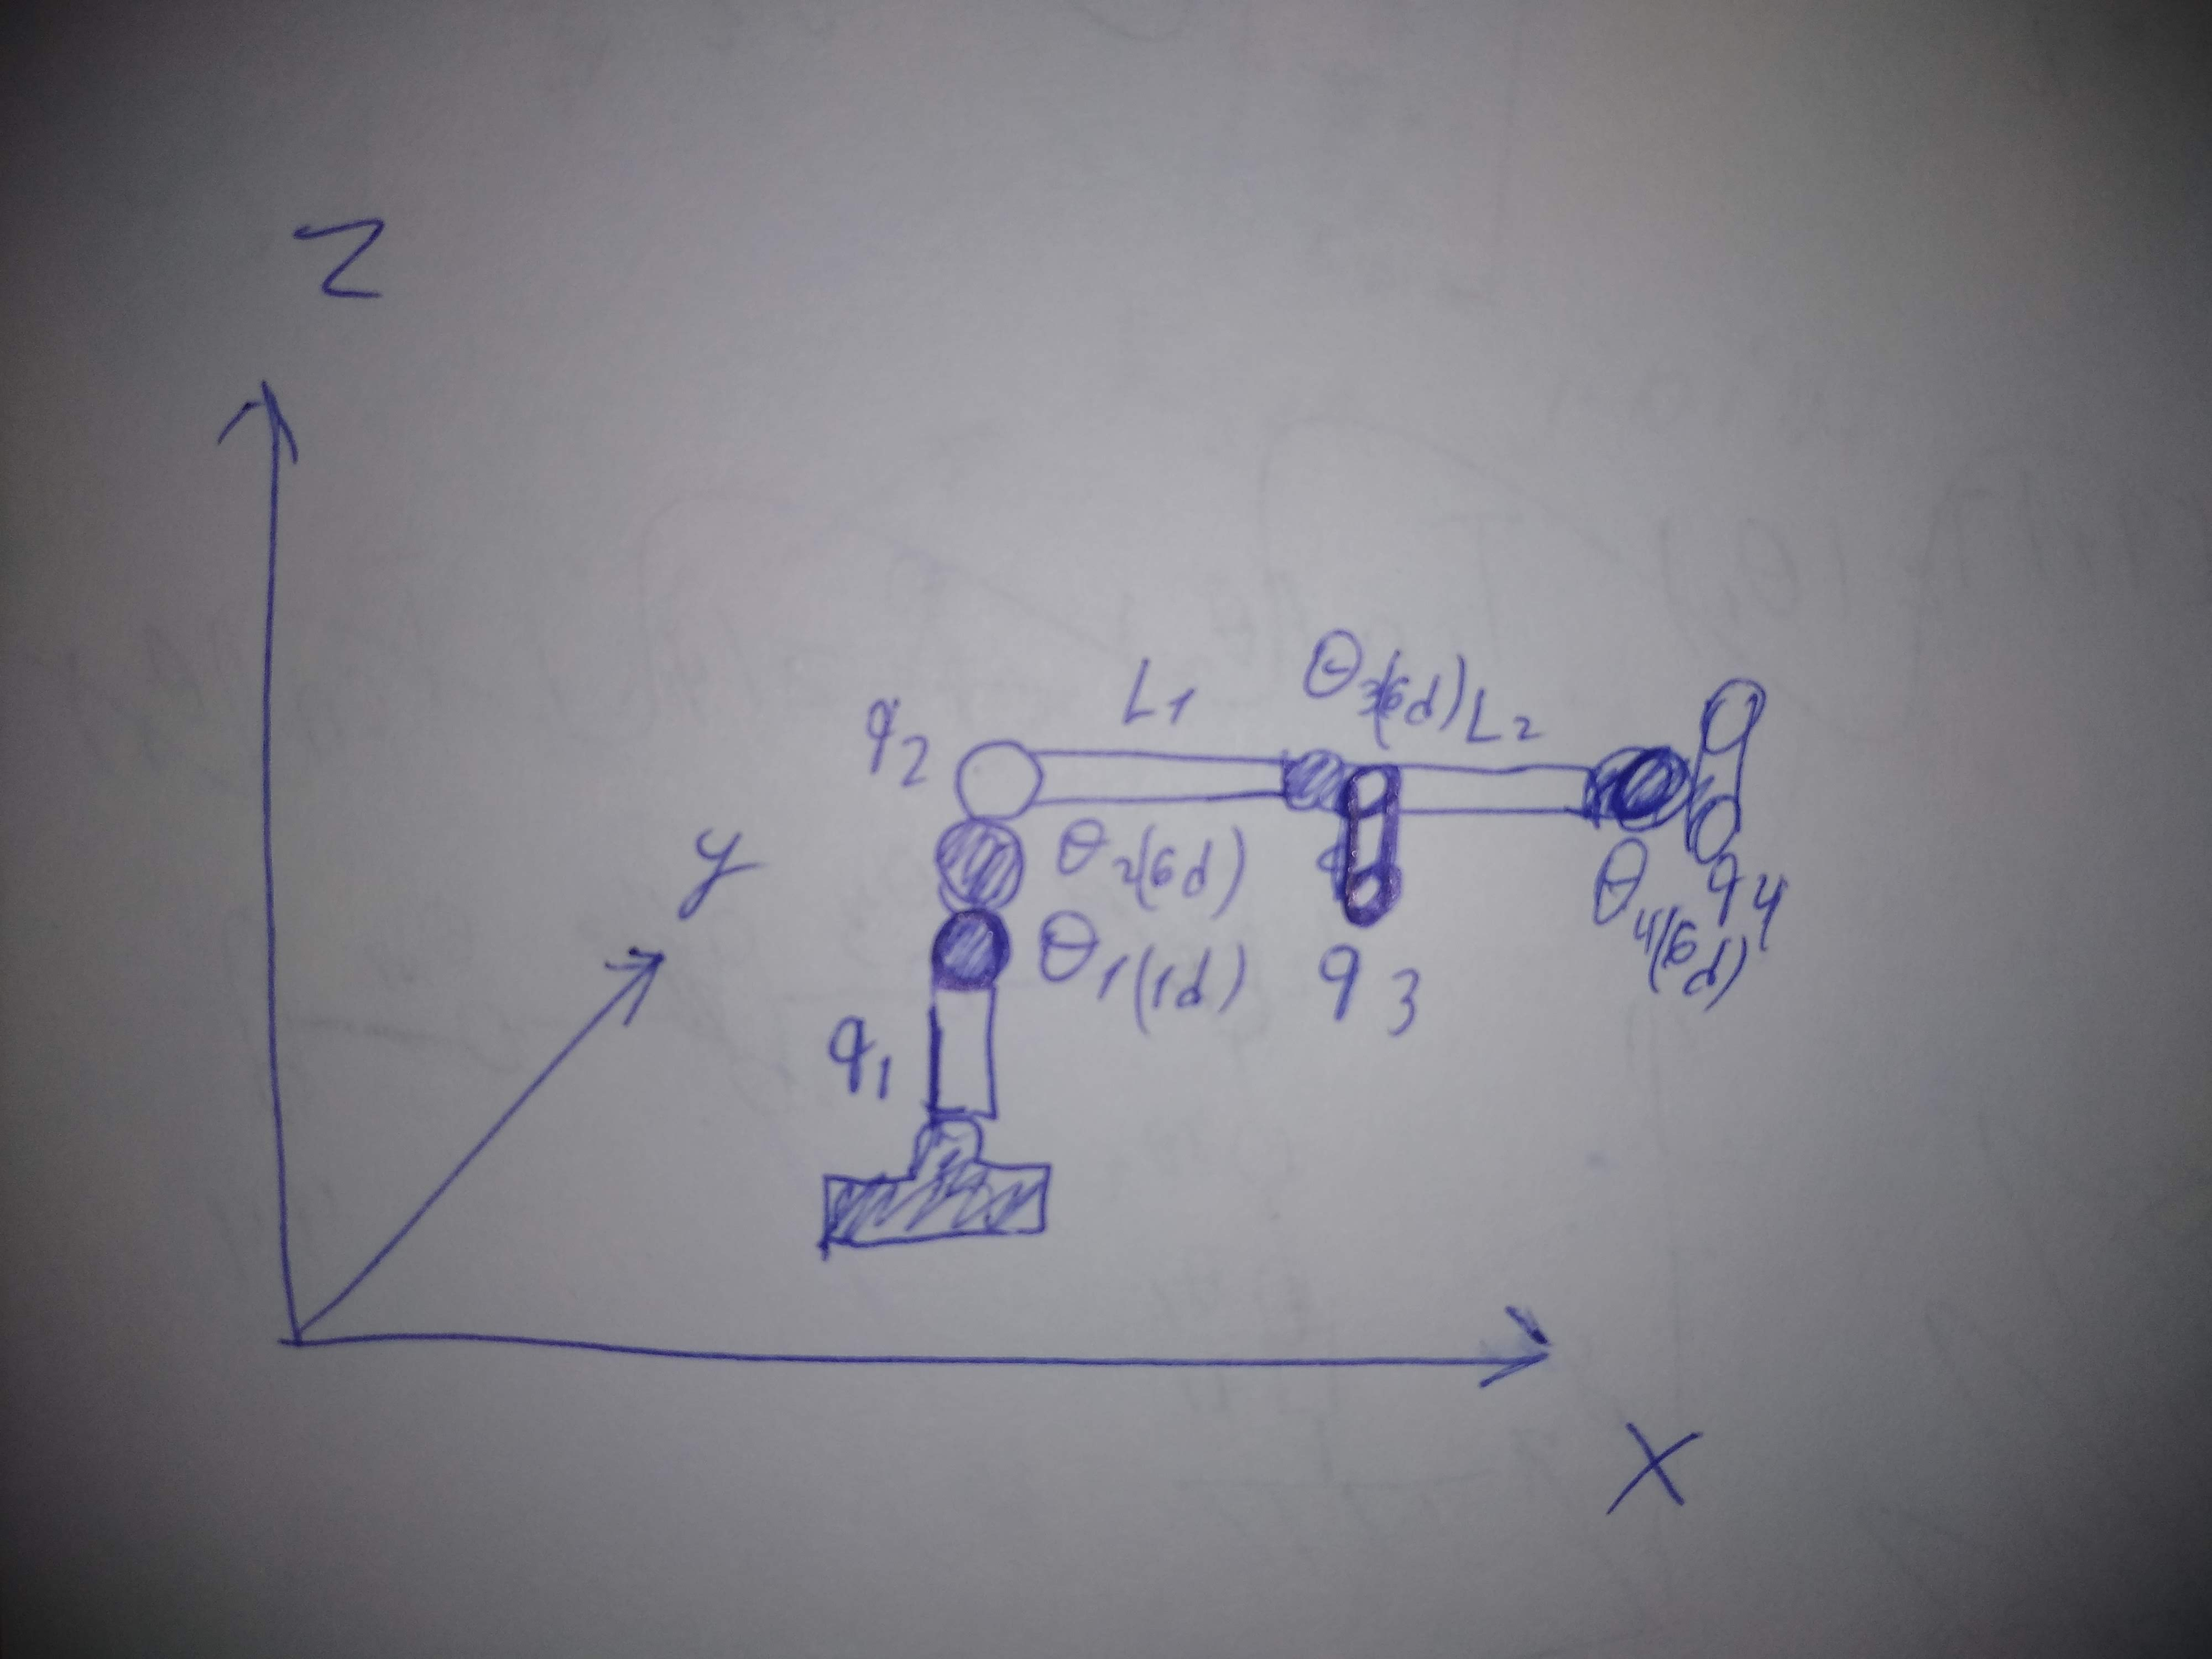
\includegraphics[scale=0.1]{scheme.jpg}
		\end{figure}
		
		\item Inverse kinematics for one leg:
		\begin{itemize}
			\item z coordinate defined by a prismatic joint position $q_1$ = z
			\item $q_2$ and $q_3$ can be found as inverse kinematics for planar 2d manipulator: \\
			\begin{math}
				q_3 = \arccos(\frac{x^2 + y^2 - L_1^2 - L_2^2}{2 L_1 L_2}) \\
				q2 = \arctan(\frac{y}{x}) - \arctan(\frac{L_2 \sin(q_3)}{L_1 + L_2 \cos(q_3)})
			\end{math}
		\end{itemize}
		
		\item For every leg there are 4 virtual joints. One is 1d (after active prismatic joint) and 3 6d (after each link).
		
		\item So the direct kinematics for this robot can be written as follows: \\
		\begin{math}
			T = T_{z}(q_1)T_{z}(\theta _{1})T_{6d}(\theta _{2})R_{z}(q_2)T_{x}(L_1)T_{6d}(\theta _3)R_z(q_3)T_x(L_2)T_{6d}(\theta _4)R_z(q_4)
		\end{math}
		
		\item After that we construct $K_\theta$ matrix base on arbitrarily chosen values of stiffness properties of links and active joints
		
		\item Then build deflection map for the robot by measurement end-effector displacement in some set of points x, y (z chose as constant since end-effector move on one plane). X and Y were taken in range from 0.1 to 1 with step 0.01:
		\begin{enumerate}
			\item For each point compute inverse kinematics of each leg assuming that virtual joints positions are 0 (since they are small)
			
			\item Compute Jacobians by virtual joints positions $J_\theta$ and passive joints $J_q$ for each leg
			
			\item Compute stiffness matrix $K$ for each leg
			
			\item Compute stiffness matrix $K_C$ of whole robot by taking sum of stiffness of all three legs
			
			\item Compute end-effector displacement: $\Delta t = K_C^{-1}W$
			
		\end{enumerate} 
		\item Deflection map on x axis plot when force applied on x (dependent on x, y position of end-effector): 
		
		\begin{figure}[H]
			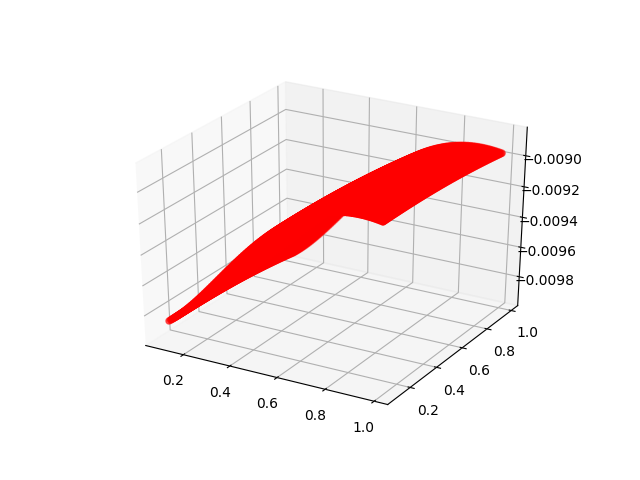
\includegraphics[scale=0.5]{x1.png}
		\end{figure}
		\begin{figure}[H]
			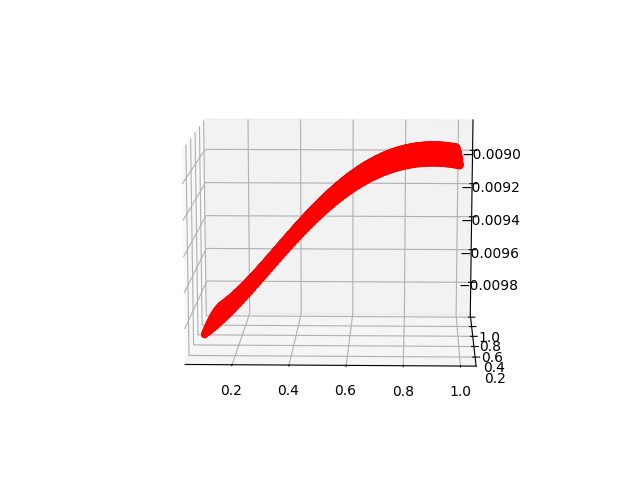
\includegraphics[scale=0.5]{x2.png}
		\end{figure}
		\begin{figure}[H]
			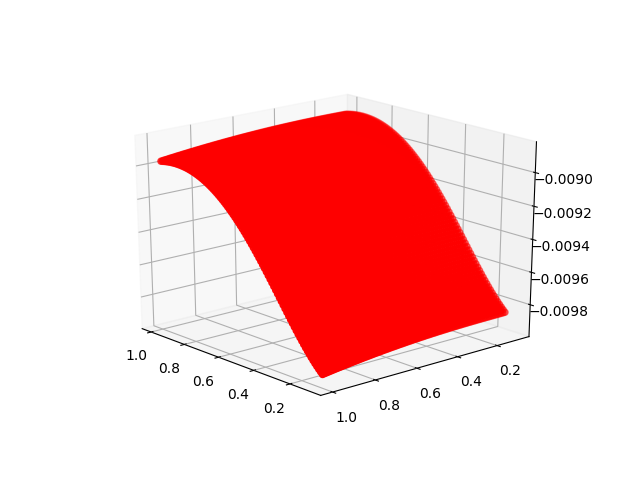
\includegraphics[scale=0.5]{x3.png}
		\end{figure}
		
		\item Deflection map by y axis plot when force applied on y (dependent on x, y position of end-effector): 
		
		\begin{figure}[H]
			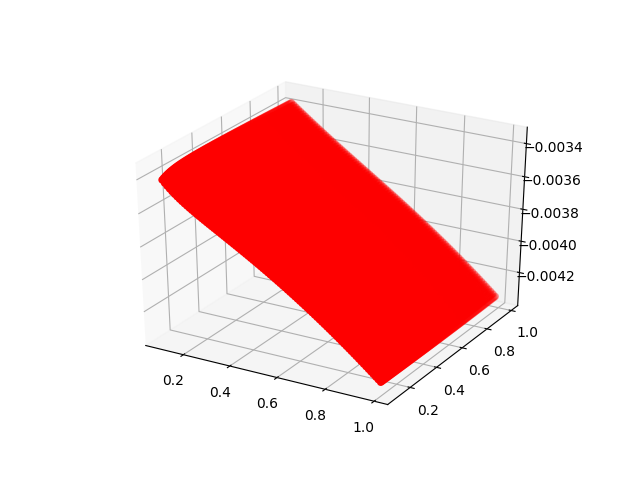
\includegraphics[scale=0.5]{y1.png}
		\end{figure}
		\begin{figure}[H]
			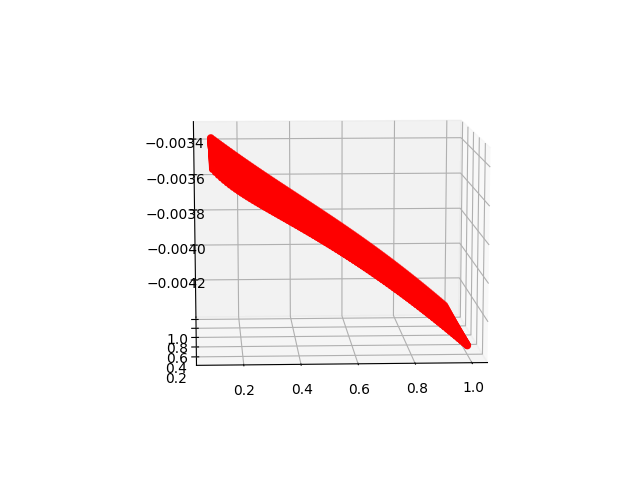
\includegraphics[scale=0.5]{y2.png}
		\end{figure}
	
		\item Deflection map by z axis plot when force applied on z (dependent on x, y position of end-effector): 
		
		\begin{figure}[H]
			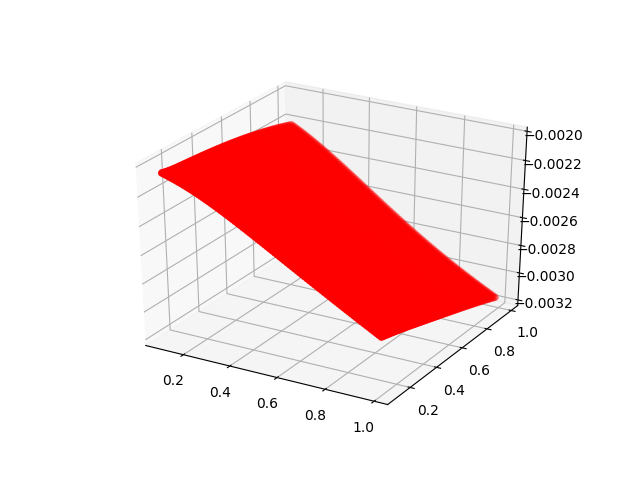
\includegraphics[scale=0.5]{z1.png}
		\end{figure}
		\begin{figure}[H]
			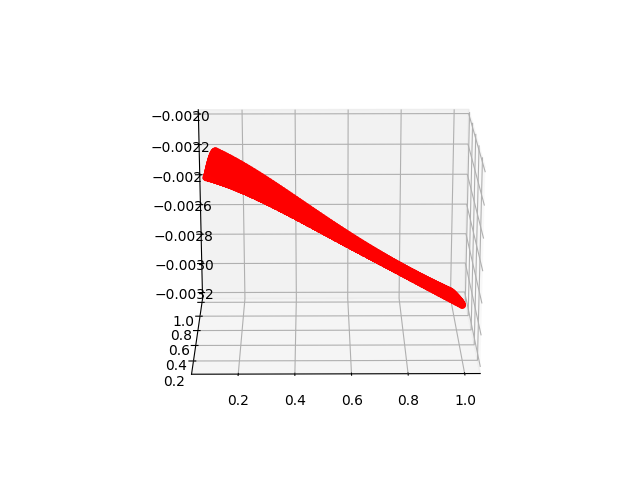
\includegraphics[scale=0.5]{z2.png}
		\end{figure}
	
	\end{itemize}

	\section{Github link:} 
	https://github.com/jenamax/Robotics_Systems/tree/master/Homework1
\end{document}